
%----------------------------------------------------------------------------------------------------------------------------------------

% définit le type de document et ses options
\documentclass[a4paper,10pt]{article}

% des paquetages indispensables, qui ajoutent des fonctionnalites
\usepackage[utf8]{inputenc}
\usepackage{graphicx}
\usepackage{lscape}
\usepackage{url}
\usepackage{xspace}
\usepackage[francais]{babel}
%\usepackage{fullpage}

\pagestyle{plain}


%----------------------------------------------------------------------------------------------------------------------------------------


% le debut du contenu
\begin{document}


%----------------------------------------------------------------------------------------------------------------------------------------


%%%%%%%%%%%%%%%%%%%%%%%%%%%%%%%%%%%%%%%%%%%%%%%%%
%%Page d'accueil
\begin{center}
	%%
	\hspace{3cm}
	
\includegraphics[scale=0.8]{logo.ps}

	%%
	\vspace{1cm}
	{\large Projet de spécialité 2010}\\
	{\Large Conception d'un modèle de feu 3D temps réel}\\
	\vspace{1cm}


	\includegraphics[scale=0.3]{feu.ps}\\
	\vspace{2cm}
	%%
	Etudiants impliqués :\\
	Benjamin Aupetit - IRVM - benjamin.aupetit@ensimag.imag.fr\\
	Julien Champeau - IRVM - julien.champeau@ensimag.imag.fr\\
	Arnaud Emilien - IRVM - arnaud.emilien@ensimag.imag.fr\\
	~\\
	Encadrants :\\
	Marie-Paule Cani  -  Marie-Paule.Cani@inrialpes.fr \\
	Aurélie Catel - aurelie.catel@grenoble-inp.fr
	~ \\
	\vspace{3mm}
	Ensimag 2010\\

\end{center}

\newpage

\tableofcontents

\newpage



%----------------------------------------------------------------------------------------------------------------------------------------
%%%%%%%%%%%%%%%%%
\section{Présentation du projet}
\subsection{Introduction}

\subsection{Objectifs}


\subsection{Aperçu}


\subsection{Analyses Bibliographiques}
%%%%%%%%%%%%%%%%%
Cette section regroupe les différents articles lus, concernant les travaux déjà effectués dans ce domaine. 
Nous allons expliquer brièvement de quoi ils parlent, ce que nous en avons retenu de bien ou de mal, ce que nous allons 
utiliser...

\subsubsection{Real-Time Fluid Dynamics for Games}
\textbf{Auteur(s)} : Jos Stam.\\
\textbf{Publication} : Proceedings of the Game Developer Conference, March 2003 \\
\textbf{Sujet(s) abordé(s)} : \\Modèle de fluide temps réel, pouvant être utilisé pour le feu, la fumée\\
	Le modèle gère: le deplacement du fluide, la gestion de combustible,les forces appliquées sur le fluide.\\	
\textbf{Principe} :\\
	Le modèle a été décomposé sur plusieurs étapes : génération du fluide par des sources, ajout des forces, diffusion du 		fluide, puis résolution de l'équation de la densité et de l'équation de la vitesse (équations de Navier-Stockes).
	Pour résoudre les deux équations, il utilise une astuce permettant de résoudre le système très rapidement.
	Enfin, il utilise le principe de conservation de la masse, qui rajoute des effets réalistes de vortex, avec la 		décomposition de Hodge.\\
\textbf{Point(s) positif(s)} :\\
	Temps réel.\\
	C'est facile à implémenter (moins de 100 lignes pour la version 2D)\\
	Peut être adapté pour la propagation du feu.\\
	Peut être adapté pour qu'un objet influe sur le modèle.\\
	Résultat réellement joli et réaliste.\\
	Très bien expliqué.\\
	Il a fournit un exemple 2D pour de la fumée, plutôt impréssionant.\\
	Le modèle peut s'adapter au feu, à la fumée, et à l'eau.\\
\textbf{Point(s) négatif(s)} :\\
	La zone d'influence est assez petite, il faut voir si c'est possible de l'étendre sans trop allourdir les calculs. (Octree?) \\
	Pas trop de détails sur la représentation graphique du feu.\\	
	La dissipation numérique implique que le résultat n'est pas exact.\\
\textbf{Conclusion} :\\
	C'est sans doute ce que nous allons adapter, pour qu'il serve à la fois pour le feu, la fumée, et la propagation.

\subsubsection{Stable Fluids}
\textbf{Auteur(s)} : Jos Stam.\\
\textbf{Publication} : SIGGRAPH 99 Conference Proceedings\\
\textbf{Sujet(s) abordé(s)} : Résolution de l'équation des fluides ( Navier-Stockes) avec, pour la première fois, un algorithme inconditionnellement stable.\\
\textbf{Principe} :\\
C'est une résolution de Navier-Stockes orientée "Computer Graphic", dans le sens o`u la résolution n'est pas exacte, et ne serait pas utilisable pour des vraies simulations de fluides, mais est "graphiquement adaptée" au problème de fluides.\\
Résolution en quatre étapes : ajout des forces, advection, diffusion, conservation de la masse.\\
\textbf{Point(s) positif(s)} : \\
2D et 3D.\\
Facile à implémenter.\\
Résolution stable et temps réel.\\
Résultat réaliste.\\
\textbf{Point(s) négatif(s)} :\\
La dissipation numérique implique que le résultat n'est pas exact.\\
\textbf{Conclusion} :\\
Ce modèle de fluide semble le plus adapté si nous choisissons d'utiliser un modèle de fluide pour le feu, la fumée et la propagation.


\subsubsection{An Interactive Simulation Framework for Burning Objets}
\textbf{Auteur(s)} : Zeki Melek, John Keyser.\\
\textbf{Publication} :\\
\textbf{Sujet(s) abordé(s)} : \\
\textbf{Principe} :\\	
\textbf{Point(s) positif(s)} :\\
\textbf{Point(s) négatif(s)} :\\
\textbf{Conclusion} :\\


\subsubsection{Visual Simulation of Smoke}
\textbf{Auteur(s)} : Ronald Fedkiw, Jos Stam, Henrik Wann Jensen.\\
\textbf{Publication} : SIGGRAPH 2001 Conference Proceedings \\
\textbf{Sujet(s) abordé(s)} : \\
	Création d'un modèle de fumée, basé sur le travail de Stam ( Stable Fluids ).\\
	Rendu réaliste de la fumée.\\
\textbf{Principe} :\\	
	L'équation du fluide est résolue comme dans "Stable Fluids". Cette fois la chaleur est prise en compte, et traitée de la même manière que la densité. Il en résulte une force de préssion qui s'ajoute simplement au modèle. Le modèle prend en compte les petits phénomènes de vortex qui se créent dans le fluide, basée sur la méthode de Steinhoff ("Vorticity confinement"). Ainsi ils rajoutent une force de rotation pour créer les minis vortex.\\
Pour le rendu : ils découpent la grille de voxels en plusieurs plans, rendus comme une superposition de plans transparents.
Une autre méthode de rendu, plus réaliste, utilise une méthode de lancé de rayons.\\
\textbf{Point(s) positif(s)} :\\
	Gestion de la chaleur.\\
	Rendu très réaliste de la fumée.\\
\textbf{Point(s) négatif(s)} :\\
	Pas en temps réel.\\
\textbf{Conclusion} :\\
	La méthode de rendu semble interessante. De plus la création de minis vortex est un atout pour le côté réaliste du modèle.

\subsubsection{Simulating Water and Smoke with an Octree Data Structure}
\textbf{Auteur(s)} : Frank Losasso, Frédéric Gibou, Ron Fedkiw.\\
\textbf{Publication} : SIGGRAPH 2004\\
\textbf{Sujet(s) abordé(s)} : \\
	Simulation d'eau et de fumée. L'équation de Navier-Stockes est résolue sur une grille Octree.\\
	La grille du modèle de fluide s'adapte selon le niveau de détail du phénomène ( par exemple plus de détails là o`u il y a des minis vortex)\\
\textbf{Principe} :\\	
	Le calcul de l'équation des fluides est effectué sur un Octree.\\
\textbf{Point(s) positif(s)} :\\
	L'octree n'est pas restreint ( ce qui était le cas des travaux précédents ).\\
	Réduction des calculs de 75\% pour un résultat équivalent avec une grille à pas constant.\\
\textbf{Point(s) négatif(s)} :\\
	Pas temps réel.\\
	Compliqué à mettre en place.\\
\textbf{Conclusion} :\\
	La complexité de la programmation est assez importante. L'avantage de cette méthode est d'avoir un très haut niveau de détail en effectuant plus de calculs là o`u cela est nécessaire. La précision que nous désiront n'est peut être pas suffisante pour nécessiter un tel modèle.



\subsubsection{Real-Time Simulation of Deformation and Fracture of Stiff Materials}
\textbf{Auteur(s)} : Matthias Müller, Leonard McMillan, Julie Dorsey, Robert Jagnow.\\
\textbf{Publication} : EUROGRAPHICS 2001 Computer Animation and Simulation Workshop \\
\textbf{Sujet(s) abordé(s)} : \\
	Destruction réaliste et temps réel d'un objet. 
\textbf{Principe} :\\	
	C'est la simplification d'un problème de propagation en négligeant les effets microscopiques, qui ne sont pas vraiment visibles en temps réel, mais coûtent énormement en calcul.\\
	Les meshs sont représentés par des "tetrahedral meshes". Le modèle de propagation continu est transformé en modèle discret. L'élasticité des objets est prise en compte.
\textbf{Point(s) positif(s)} :\\
	Temps réel.\\
	Le système est stable est rapide.\\
	La méthode de destruction de l'objet basée sur des tétrahèdres est très intéressante.\\
	Propagation des effets de la destruction à l'intérieur de l'objet.\\
\textbf{Point(s) négatif(s)} :\\
	Peut être lourd à utiliser si il y a trop d'objets à l'écran.\\
\textbf{Conclusion} :\\
	Le principe de déformation sur un mesh tétrahédral est très intéressant, et peut facilement s'adapter à un modèle de fluide.



\subsubsection{Voxels On Fire}
\textbf{Auteur(s)} : Ye Zhao, Xiaoming Wei, Zhe Fan, Arie Kaufman, Hong Qin.\\
\textbf{Publication} :\\
\textbf{Sujet(s) abordé(s)} : \\
\textbf{Principe} :\\	
\textbf{Point(s) positif(s)} :\\
\textbf{Point(s) négatif(s)} :\\
\textbf{Conclusion} :\\

\subsubsection{Meshes On Fire}
\textbf{Auteur(s)} : Haeyoung Lee, Laehyun, Mark Meyer, Mathieu Desbrun.\\
\textbf{Publication} : Eurographics Workshop on Computer Animation and Simulation '2001 \\
\textbf{Sujet(s) abordé(s)} : \\
	Propagation des flammes à la surface d'un objet.\\
\textbf{Principe} : \\
	La propagation est un parcours géodésique de la surface, et subit le vent environnant.\\	
	Les flammes sont rendues sont formes de particules avec des blobs.\\
	Les flammes générées subissent le champ de vent ce qui les rend plus réaliste.\\
\textbf{Point(s) positif(s)} :\\
	Temps réel.\\
	Prise en compte de plusieurs feu.\\
	Rapide à calculer.\\
	Très efficace pour changer la texture d'un objet brulé.\\
	Propagation fonction d'un champ de vent.\\
	Les particules de feu générées peuvent être utilisées pour génerer un feu sur un autre objet ou sur une autre partie de l'objet.\\
\textbf{Point(s) négatif(s)} :\\
	Ne peut pas s'adapter à la destruction d'un objet.\\
	Peut être une perte de performance si on utilise les particules de feu pour allumer des foyer aux autres endroits du mesh.\\
	La propagation surfacique n'est pas toujours adaptés.\\	
\textbf{Conclusion} :\\
	Ce modèle est interessant, mais nécessite d'être beaucoup modifié pour correspondre à notre but. Il n'est pas très adapté à la destruction des objets. (Sauf si nous voulons uniquement dégrader la texture de l'objet) \\

\subsubsection{Real-time Procedural Volumetric Fire}
\textbf{Auteur(s)} : Alfred R. Fuller, Hari Krishnan, Karim Mahrous, Bernd Hamann, Kenneth I. Joy.\\
\textbf{Publication} : Proceedings of the 2007 symposium on Interactive 3D graphics and games\\
\textbf{Sujet(s) abordé(s)} : \\
	Rendu de feu réaliste en temps réel, utilisant le bruit de perlin.
\textbf{Principe} :\\
	La flamme est calculée en 3 dimensions, et le rendu est effectué par le GPU.\\
	L'animation de la texture est procédurale.\\	
\textbf{Point(s) positif(s)} :\\
	Temps réel.\\
	Réaliste.\\
\textbf{Point(s) négatif(s)} :\\
	Représentation du feu uniquement, pas de propagation et de fumée.\\
\textbf{Conclusion} :\\
	La qualité du feu est importante, mais ce modèle de flamme ne concerne que la partie "affichage". Il faudra voir si le modèle de propagation choisi peut utiliser un tel modèle de flammes.



%----------------------------------------------------------------------------------------------------------------------------------------
%%%%%%%%%%%%%%%%%
\section{Mise en place du modèle global}
%%%%%%%%%%%%%%%%%




%----------------------------------------------------------------------------------------------------------------------------------------
%%%%%%%%%%%%%%%%%
\section{Modèle de flamme}
%%%%%%%%%%%%%%%%%





%----------------------------------------------------------------------------------------------------------------------------------------
%%%%%%%%%%%%%%%%%
\section{Modèle de fumée}
%%%%%%%%%%%%%%%%%





%----------------------------------------------------------------------------------------------------------------------------------------
%%%%%%%%%%%%%%%%%
\section{Propagation sur l'objet}
%%%%%%%%%%%%%%%%%





%----------------------------------------------------------------------------------------------------------------------------------------
%%%%%%%%%%%%%%%%%
\section{Destruction de l'objet}
%%%%%%%%%%%%%%%%%





%----------------------------------------------------------------------------------------------------------------------------------------
%%%%%%%%%%%%%%%%%
\section{Propagation dans l'environnement}
%%%%%%%%%%%%%%%%%


%----------------------------------------------------------------------------------------------------------------------------------------
%%%%%%%%%%%%%%%%%
\section{Références}
%%%%%%%%%%%%%%%%%


%----------------------------------------------------------------------------------------------------------------------------------------
\end{document}
